Similar to time-domain IIR architecture, a feedback is required to generate the recursive part of the response. For example in Fig.~\ref{fig_IIRBasicArch}, we show a second order IIR filter, where weighted and delayed versions of the input signal $x$ are fed back to the  input.  
\begin{figure}[t!]
    \begin{center}
        \begin{overpic}[width=0.65\linewidth, 
        % grid, 
        tics=10,trim=0 0 0 0]{./Media/BASIC_IIR_FILTER_ARCH.png}
            \put (60, 50){\footnotesize{$\beta_{0}$}}
            \put (60, 30){\footnotesize{$\beta_{1}$}}
            \put (60, 10){\footnotesize{$\beta_{2}$}}
            \put (36, 30){\footnotesize{$\alpha_{1}$}}
            \put (36, 10){\footnotesize{$\alpha_{2}$}}
            \put (10, 50){\footnotesize{$x$}}
            \put (85, 50){\footnotesize{$y$}}
            \put (47.5, 34.5){\footnotesize{$z^{-1}$}}
            \put (47.5, 14.5){\footnotesize{$z^{-1}$}}
        \end{overpic}
    \end{center}
    \caption{Direct form II $2^{nd}$ order IIR architecture.}
    \label{fig_IIRBasicArch}
\end{figure}
In order to do so in the spatial domain, we propose a dual beam-former architecture (see Fig.~\ref{fig:Proposed_spatialIIR_ARCH}), defined by two sets of weights $\vBeta$ and $\vAlpha$.
The beamformed signal, $\sum_{n}x_{n,\theta_g}(t)\beta_n$, can be seen as with classical beamforming while the weights $\vAlpha$ generate the recursive part of the response by re-transmitting the received array signals $\Brace{x_{n,\theta_g}}$ and the input $x(t)$ back to the target. 
\begin{figure}[t!]
    \begin{center}
        \begin{overpic}[width=0.8\linewidth, 
        % grid, 
        tics=10,trim=0 0 0 0]{./Media/SpatialIIR-diagram/SpatialIIR_VER6.png}
            \put (3.5, 25){\footnotesize{$\beta_{0}$}}
            \put (14.5, 25){\footnotesize{$\beta_{1}$}}
            \put (37, 25){\footnotesize{$\beta_{N-1}$}}
            \put (48, 25){\footnotesize{$\alpha_{0}$}}
            \put (59.5, 25){\footnotesize{$\alpha_{1}$}}
            \put (85, 25){\footnotesize{$\alpha_{N-1}$}}
            \put (29, 53){\footnotesize{$d$}}
            \put (91.5, 87){\footnotesize{$p_{t}$}}
            \put (60, 40){\footnotesize{$p_{N-1}$}}
            \put (37, 40){\footnotesize{$p_{1}$}}
            \put (25.5, 40){\footnotesize{$p_{0}$}}
            \put (46, 52){\footnotesize{$\theta_{g}$}}
            \put (17.5, 12){\footnotesize{$\Sigma$}}
            \put (62, 12){\footnotesize{$\Sigma$}}
            \put (43.5, 12){\footnotesize{$x\rBrace{t}$}}
            \put (32.2, 12){\footnotesize{$n\rBrace{t}$}}
            \put (20,5){\footnotesize{$y\rBrace{t}$}}
        \end{overpic}
    \end{center}
    \caption{The proposed ``dual beam-former" architecture. The weights $\vBeta$ generate the output signal $y(t)$. The  weights $\vAlpha$ synthesize the feedback transmission.
    $x(t)$ is the input waveform which is transmitted together with the feedback beamformed signal.
    An additive noise model $n\rBrace{t}$ is assumed at the array output.}
    \label{fig:Proposed_spatialIIR_ARCH}
\end{figure}
\subsection*{Obtained spatial response}
\myTodo{inline} {this is not clear. \\
\textbf{DONE}\\Please write the propagation model: $x_{n=0,\theta}=...$ actually this is like eq(1) but we need to add the attenuation g there. Note that g should depend on the angle, and the index of the antenna $g=g_{n,\theta}$. Only if there is no choice, we can assume isotropic antennas such that this dependency can be removed. 
\\\textbf{DONE:}\\Also, if $g$ represents the total attenuation (up link+down link+antenna gain in that specific direction) we do not need to write $g^2$. 
\\\textbf{DONE:}\\Also, use the notations $x_{n,\theta}$ within eq(2).
\\\textbf{DONE:}\\Also, I dont think eq (2) is exact. Why have you added the $n\tau_\theta$ in the second (sum) term? 
\\\textbf{DONE:}\\Also, start with general manifold and plug in the ULA only at the end as a special case.}
Time domain analysis of the proposed feedback based architecture, considering both propagation delay and attenuation, gives rise to
\begin{equation}
    \label{eqn:SingleSensorTemporalEquality}
    % \resizebox{.91\linewidth}{!}{
        \begin{split}
            x_{n}(t) = g\rBrace{s\rBrace{t-\tau_{pd}-\tau_{n}}
            +\sum_{m=0}^{N-1}{\alpha_{m}x_{m}\rBrace{t-\tau_{pd}-\tau_{n}}}},
        \end{split}
    % }
\end{equation}
where the first term of the right-hand side represents the contribution of the transmitted waveform $s(t)$ to the $n$'th array element and the second term represents the feedback contribution of the re-transmitted array signal to this same element.
Expressing \eqref{eqn:SingleSensorTemporalEquality}'s Fourier transform,
\begin{equation}
    \label{eqn_singleSensorFourier}
    % \resizebox{.91\linewidth}{!}{
        \begin{split}
            \F{x}_{n}\rBrace{\omega} =
            g\Bigg( & \F{s}\rBrace{\omega}
            \exp\rBrace{-j\omega\rBrace{\tau_{pd}+\tau_{n}}}
            \\&+\sum_{m=0}^{N-1}
            {
            \alpha_{m}\omegaB\F{x}_{m}\rBrace{\omega}
            \exp\rBrace{-j\omega\rBrace{\tau_{pd}+\tau_{n}}}
            }\Bigg),
        \end{split}
    % }
\end{equation}
and its vector from,
$$
\F{\vx}\rBrace{\omega} = ge^{-j\omega\tau_{pd}} \rBrace{\F{s}\rBrace{\omega}+\vAlphaT \F{\vx}\rBrace{\omega}}\vd,
$$
we find that it can be simplified to
$$
\F{\vx}\rBrace{\omega} =\rBrace{I-g\vd\vAlphaT{}e^{-j\omega\tau_{pd}}}^{-1}g\vd\exp{\rBrace{-j\omega\tau_{pd}}}\F{s}\rBrace{\omega}.
$$
Then, denoting
\[
\phi\triangleq\omega\tau_{pd}
\]
as the round-trip signal propagation related electrical phase and using the Woodbury matrix identity \cite{woodbury1950inverting}, we find that
$$
\F{\vx}\rBrace{\omega}
=
\frac{    
g\vd\exp{\rBrace{-j\phi}}
}{
1 - g\aTd{}\exp{\rBrace{-j\phi}}
}\F{s}\rBrace{\omega}.
$$
Considering the noiseless case $\rBrace{\text{i.e. n}\rBrace{t}=0}$,
we express the general spatial response of FB as 
\begin{equation}
\label{eqn:GeneralFeedbackTransferFunction}
\Hba
\triangleq
\frac{\F{z}\rBrace{\omega}}{\F{s}\rBrace{\omega}} 
=
\frac{    
g\bTd{}\exp\rBrace{-j\phi}
}{
1 - g\aTd{}\exp\rBrace{-j\phi}
}.
\end{equation}
\par Note that this result confirms that the suggested architecture achieves a controllable (via setting of $\vBeta$ and $\vAlpha$) and recursive (non-trivial denominator) spatial response.
As will be shown, high directivity and narrow beam-width are obtainable by proper selection of the weights. Comparing to traditional beamformers (i.e. with no feedback), the performance improvement will be expressed in terms of aperture increase, computing the traditional beamformer aperture which achieves the same performance.
One may observe that opposed to traditional beamformers, the beampattern, $\Hba,$ is not only influenced by the impinging signal DOA, for it is also range selective due to its $\phi$ dependency.
As exemplified in Fig.~\ref{fig_rangeAzimuthSelectivity}, the combination of both angular and range selectivity enables the designer to enhance signals arriving from specific locations rather than only specific directions.
\begin{figure}[t!]
    \begin{center}
        \begin{overpic}[width=0.65\linewidth, 
        % grid, 
        tics=10,trim=0 0 0 0]{./Media/azimuthRangSelectivity.png}
            \put (20, 23){\rotatebox{0}{\footnotesize{Angular response}}}
            \put (30.5, 47){\rotatebox{0}{\footnotesize{Enhanced radial slice}}}
        \end{overpic}
    \end{center}
     \caption{A visualization of the spatial area selectivity concept. Combining both radial selectivity (i.e. enhancing signals from a specific distance) and DOA-based selectivity, allows the enhancement of signals arriving from specific areas (grey filled), while signals originated in other areas (even from the same DOA) are suppressed.}
    \label{fig_rangeAzimuthSelectivity}
\end{figure}
\section{Fisher Information Matrix}
\label{sec_FIM}
A possible evaluation for the contribution of the presented feedback mechanism is to measure the additional information in the system.
To this end, the FIM, denoted by $J$, will now be calculated with respect to the DOA parameter $\thetaD$ and the range related parameter $\phi$. 
As the feedback-based transfer function (\ref{eqn:GeneralFeedbackTransferFunction}) is expressed in frequency domain, we rely on \cite{zeira1990frequency} to express the frequency domain FIM as well. 
\par A single FIM element, may be expressed as
\begin{equation}\label{eq_FIM_kl_full}
    \resizebox{.9\linewidth}{!}{
        \begin{split}
            J_{\vBrace{k,l}}\rBrace{\vEta} 
            =&
            \Re\cBrace{
            \frac{1}{2\pi}
            \int_{-\omega_{s}/2}^{\omega_{s}/2}
            {
            \frac{1}{\Phi\rBrace{\omega}}
            \mathfrak{F}^{*}\left\{
            \frac{\partial z(t)}{\partial\eta_{k}}
            \right\}
            \mathfrak{F}\left\{
            \frac{\partial z(t)}{\partial\eta_{l}}
            \right\}
            d\omega
            }}
            \\ &+
            \frac{T}{4\pi}
            \int_{-\omega_{s}/2}^{\omega_{s}/2}
            \frac{1}{\Phi^{2}\rBrace{\omega}}
            \frac{\partial\Phi\rBrace{\omega}}{\partial\eta_{k}}
            \frac{\partial\Phi\rBrace{\omega}}{\partial\eta_{l}}
            d\omega
        \end{split}
    }
\end{equation}
where $ \vEta = [\thetaD,\phi]^{T} $ is the parameters vector, $\Re$ stands for the real-part extraction operator, $k,l \in\cBrace{1,2}$, $\Phi\rBrace{\omega}$ is the noise spectrum, $\mathfrak{F}$ is the Fourier transform operator, $T$ is the measurement observation interval and $\omega_{s}$ is the signal bandwidth. 
For simplicity, $\text{n}\rBrace{t}$ is assumed to be a white Gaussian with some constant power spectral density $\Phi(\omega)=\sigma^2$ and independent of the estimated parameters $\eta$, hence the second term vanishes. 
Assuming continuously differentiable functions, where order alteration of the Fourier transform and the differentiation operations is allowed, \eqref{eq_FIM_kl_full} simplifies to
\begin{equation}
    \label{eq_beamPatternFreqDomain_FIM}
    % \resizebox{1\linewidth}{!}{
        \begin{split}
            J_{\vBrace{k,l}}\rBrace{\vEta} = 
            \Re\cBrace{
            \frac{1}{2\pi\sigma^2}
            \int_{-\omega_{s}/2}^{\omega_{s}/2}
            {
            \rBrace{\frac{\partial{}\F{z}\rBrace{\omega}}{\partial\eta_{k}}}^{\ast}
            \frac{\partial{}\F{z}\rBrace{\omega}}{\partial\eta_{l}}
            d\omega
            }}
        \end{split}.
    % }
\end{equation}
As mentioned before, $g$ is independent of the estimated parameters, therefore
\begin{equation}\label{eq_vdDiff}
\frac{\partial\vd}{\partial\thetaD}=A\omegaB\vd
\end{equation}
where $A\omegaB$ is an $N\times{}N$ diagonal matrix and each of its diagonal elements may expressed as 
\[
A_{\vBrace{i,i}}\omegaB=-j\omega\frac{\partial \tau_{i}}{\partial{\thetaD}}\ \  \forall{i\in\cBrace{0\hdots{}N-1}}.
\]
To further simplify the analysis, without loss of generality, we use (in this section only) $g=1$.
In App.~\ref{apdx_clacFim} we compute the FIM terms, concluding that
\begin{equation}
    \label{eqn_FIMelements}
    \resizebox{.91\linewidth}{!}{
        \begin{split}
            &J_{\theta\theta}
            =
            \frac{1}{2\pi\sigma^{2}}\int_{-\omega_{s}/2}^{\omega_{s}/2}{\frac{
            \lBrace{\vBetaT{}A\omegaB\vd-\vBetaT{}B\omegaB\vAlpha\ePhi{-}}^{2}
            }{
            \lBrace{\rBrace{1-\aTd\ePhi{-}}^{2}}^{2}
            }\lBrace{\F{s}\rBrace{\omega}}^{2}d\omega}
            \\
            &J_{\phi\phi}
            =
            \frac{1}{2\pi\sigma^{2}}\int_{-\omega_{s}/2}^{\omega_{s}/2}{\frac{
            \lBrace{\bTd}^{2}
            }{
            \lBrace{\rBrace{1-\aTd\ePhi{-}}^{2}}^{2}
            }\lBrace{\F{s}\rBrace{\omega}}^{2}d\omega}
        \end{split}
    }
\end{equation}
where $B\omegaB\triangleq\vd\vdT{}A\omegaB-A\omegaB\vd\vdT$.
Moreover, using some mild assumptions and setting
\begin{equation}\label{eq_alphaBetaPropSteer}
    \vAlpha,\vBeta\propto\vd^{\ast},
\end{equation}
we show that the cross terms of the FIM are nullified, i.e. $J_{\theta\phi} = J_{\phi\theta}^{*}=0$.
\par 
Choosing the weights as in \eqref{eq_alphaBetaPropSteer} may be interpreted as a generalization of the DS beamformer, formerly referenced as the conventional beamformer (CB) \cite{van2004optimum}, which coherently integrate the impinging signal along the array elements.
The same choice of weights also minimizes the $\lBrace{1-\aTd\ePhi{-}}$ term, significantly increasing the available information, as predicted by the FIM.
It is worth mentioning that \eqref{eq_vdDiff} is relevant even for arbitrary (non-omni-directional) sensors when smooth and slowly changing radiation patterns are assumed.
In practice, though, there will be unavoidable errors, and perfect knowledge of the steering vector $\vd$ is not always available.
In Sec.~\ref{sec_Performance}, we quantify the effect of such estimation errors and discuss its influence on the array performance. 
\section{Performance Analysis}
\label{sec_Performance}
In this section we analyze some of the fundamental properties of the suggested array; it's beamwidth, peak to side-lobe level and it's directivity which are all compared to traditional array processing. Focusing on ULA, we show that by integrating the spatial feedback, we obtain improved performance compared to the classic beamforming.

\myTodo{inline}{\textbf{DONE:}\\Please rephrase the following text. Maybe you meant something like: As seen from the FIM structure, large information can be obtained by setting the denominator close to zero. This implies that $\bTd g\exp\Brack{-j\phi}$ should be as close to one as possible. Assuming that we choose the beamformer weights in the form of $\alpha=\hat{g}^{-1}\exp\Brack{j\hat{\phi}}d_{\hat{\theta}}$  in order to coherently sum up the energy from a presumed direction $\hat{\theta}$, while compensating for the channel attenuation $g$ and phase $\phi$ with their estimated values. 
\\\textbf{Comment : But the steering vectors are not normalized. They consist from exponents.}
\\\footnote{we need in advance state that we assume all steering vectors are normalized ... }
\\\textbf{DONE:} 
\\I also don't like the use of this DCBF. Why not to call this coherent beamformer approach? (CB in short) }
\subsection*{Error terms}
We now focus on an $N$-element ULA, with steering vector
\[
\vd=g\sBrack{1,\exp(-\theta),\ldots,\exp(-(N-1)\theta)}^T
\]
with $\theta$ of \eqref{eq:thetaULA}, and some real gain $g$. 
Following previous observations, we  analyze the case of CB, where we coherently sum the array elements using
\begin{equation}\label{eq:alpha_beta_hat}
\vBeta_{\coefSetName{}}=\vAlpha_{\coefSetName{}}=\hat{\vd}^{\ast}\exp\rBrace{j\hat{\phi}}/\norm{\hat{\vd}}^2
\end{equation}
where 
\[
\hat{\vd}=\hat{g}\sBrack{1,\exp(-\hat\theta),\ldots,\exp(-(N-1)\hat\theta)}^T
\]
is an estimate of the steering vector, and $\hat{\phi}, \hat\theta$ are the estimates of the range-related phase, and the DOA-related phase, respectively.
Plugging \eqref{eq:alpha_beta_hat} within \eqref{eqn:GeneralFeedbackTransferFunction}, we obtain
\begin{equation*}
    \resizebox{1.01\linewidth}{!}{
        \begin{split}
            H_{\vBeta_{\coefSetName{}},\vAlpha_{\coefSetName{}}}\triangleq{}H_{\dTheta,\dPhi}\rBrace{\omega}=\frac{r\D{\dTheta/2}{N}\exp\rBrace{-j\rBrace{\dPhi+(N-1)\dTheta/2}}}{1-r\D{\dTheta/2}{N}\exp\rBrace{-j\rBrace{\dPhi+(N-1)\dTheta/2}}}
        \end{split}
    }
\end{equation*}
where \[
\D{x}{N}\triangleq\frac{1}{N}\frac{\sin\rBrace{Nx}}{\sin\rBrace{x}}
\]
is the normalized Dirichlet kernel and
we define the DOA, range and gain error terms 
\[
\dTheta\triangleq {\theta-\hat{\theta}},\ \dPhi\triangleq {\phi-\hat{\phi}},\ 
r\triangleq g/\hat{g},
\]
respectively. From here now, we shall use the $H_{\dTheta,\dPhi}$ notation, such that $H_{x,y}=H_{\dTheta=x,\dPhi=y}$.
\par We will consider the following four fundamental scenarios
\begin{itemize}
    \item{\makebox[.55\linewidth]{The perfectly aligned scenario \hfill} $\rBrace{\dTheta=0\ , \dPhi=0}$}
    \item{\makebox[.55\linewidth]{The steer error scenario \hfill} $\rBrace{\abs{\dTheta}>0\ , \dPhi=0}$}
    \item{\makebox[.55\linewidth]{The range error scenario \hfill} $\rBrace{\dTheta=0\ , \abs{\dPhi}>0}$}
    \item{\makebox[.55\linewidth]{The general scenario \hfill} $\rBrace{\abs{\dTheta}>0\ , \abs{\dPhi}>0}$}.
\end{itemize}
\ifdefined\showTodo
{
    \subsection*{Small estimation error analysis - \textbf{TO BE REMOVED - kept only for the todos}}
    \label{subsection_ArrayPerformance_TayolrAnalysis}
    \myTodo{inline}{\textbf{DONE:}\\ maybe to call this subsection 'small error analysis'}
    Plugging (\ref{eqn_CB_coefSet}) into (\ref{eqn:GeneralFeedbackTransferFunction}) and denoting $\D{N}{x} \triangleq \frac{\sin{\rBrace{Nx}}}{\sin{\rBrace{x}}}$ results in the general \coefSetName{} beampattern \myTodo{inline}{\textbf{DONE}\\you need to define the delta expressions (the errors)}
    \begin{equation*}
        h_{\coefSetName{}}\rBrace{\theta,\omega}
        =
        \frac{
        \D{N}{\dTheta/2}exp\rBrace{-j\rBrace{\dPhi+\frac{N-1}{2}\dTheta}}
        }{
        N - \D{N}{\dTheta/2}exp\rBrace{-j\rBrace{\dPhi+\frac{N-1}{2}\dTheta}}
        }.
    \end{equation*}
    For the evaluation of the various array parameters, we define the normalized beampattern \myTodo{inline}{\textbf{DONE:}\\not very readable. Consider writing a multiplication of two terms. Suggesting that you write the expression in eq(5) as $H(\theta,\phi)$ and here you'll have $H(\hat{\theta}, \hat{\phi})/ H(\theta,\phi)$}
    \begin{equation}
        \label{eqn_arrPerformance_beamwidth_3dB}
        \Hr{\theta}{\tau}{}\triangleq\fbBpRatio.
    \end{equation}
    \myTodo{inline}{\textbf{DONE:}\\this next section is very long. Suggesting that you express (10) in terms of the errors $\Delta\theta,\;\Delta\phi$, and then simply state that the second order Taylor expansion of those errors around zero gives (12). One more issue which I think might cause us some headache is that we cannot assure that $\Delta\phi$ (you call it $\Delta\tau$) is indeed close to zero, as this term fluctuates very fast. But we will think about it later on. Maybe something with wideband signal stimulus will solve this issue.}
    The pursuit for analytic dependencies between $\Hr{\theta}{\tau}{}$, $\dTheta$ and $\dPhi$, as in \cite{VanTrees2002DetectionIV}, lead to expressing $\Hr{\theta}{\tau}{}$'s multivariate Taylor expansion, setting $\dTheta,\dPhi$ as the variables. Simulations have shown that $2^{nd}$ Taylor expansion achieves very accurate results, thus we use it to express the array parameters. As commonly known, the Taylor expansion of a multivariate analyzable function $f\rBrace{\vx}$ around $\vx_{0}$ where $\vx \in \mathbb{R}_{M\times1},$ is 
    \begin{equation}
        \label{eqn_h_Tylor_dTheta_dTau}
        \evalat{f\rBrace{\vx}}{\vx\to\vx_{0}}=\sum_{n=0}^{\infty}\frac{1}{n!}\rBrace{\sum_{i=1}^{M}(x_{i}-x_{0i})\frac {\partial}{\partial x_i} }^n f(x_k)|_{x_k=x_{k0}},
    \end{equation}
    where $\frac{\partial}{\partial x_i}$ is the derivative operator and $i\in\left[1\hdots{}M\right]$. Reducing (\ref{eqn_h_Tylor_dTheta_dTau}) to its $2^{nd}$ form (i.e $f(x,y)=\sum_{n=0}^{\infty} \frac 1 {n!}\rBrace{x\frac {\partial}{\partial x}+y\frac {\partial}{\partial y} }^n f(x,y)|_{(x,y)=(0,0)}$), combined with the binomial formula, $(x+y)^{n}=\sum _{k=0}^{n}{\binom {n}{k}}x^{n-k}y^{k},$ multiple iterations of L'Hôpital's rule and algebraic simplification finally yields
    \begin{equation}
        \begin{split}
            \evalat{\Hr{\theta}{\tau}{}_{\coefSetName{}}}{\dTheta\to0,\dPhi\to0} \approx\ & 1 
            \\+&\frac{\binom{2}{0}}{2!}\frac{-\rBrace{N - 1}\rBrace{N-4r+2Nr+1}}{6\rBrace{r-1}^{2}}\dTheta^{2}
            \\+&\frac{\binom{2}{1}}{2!}\frac{-r\omega\rBrace{N - 1}}{\rBrace{r-1}^{2}}\dTheta\dPhi
            \\+&\frac{\binom{2}{2}}{2!}\frac{-2r\omega^{2}}{\rBrace{r-1}^{2}}\dPhi^{2}
        \end{split}
    \end{equation}
}
\else
\fi
\subsection*{The normalized beampattern}
\label{subsection_spatialIIR_normBP}
Common ULA array parameter analysis \cite{VanTrees2002DetectionIV}, investigates certain characteristics of normalized beampatterns (i.e. main lobe gain of $0_{dB}$) in order to achieve an objective analysis which is independent of its coefficients magnitude. Motivated by the same purpose, we define the normalized beampattern as
\begin{equation}
    \label{eqn_arrPerformance_beamwidth_3dB}
    \resizebox{.89\linewidth}{!}{
    \begin{split}
        \Hr_{\dTheta,\dPhi}&\triangleq
        \lBrace{
        \frac{
        H_{\dTheta,\dPhi}\rBrace{\omega}
        }{
        H_{0,0}\rBrace{\omega}
        }
        }^{2}
        =
        \lBrace{
        \frac{
        H_{\dTheta,\dPhi}\rBrace{\omega}
        }{
        r^{2}/\rBrace{1-r}^{2}
        }
        }^{2}
        \\
        &=\frac{\rBrace{1-r}^{2}\Dp{\dTheta/2,N}{2}}{1+r^{2}\Dp{\dTheta/2,N}{2}-2r\D{\dTheta/2}{N}\cos{\rBrace{\dPhi+\frac{N-1}{2}\dTheta}}},
    \end{split}
    }
\end{equation}
% \begin{figure*}[bh!]
%     \begin{equation}\label{eqn_generalCaseBp}
%         \resizebox{.91\linewidth}{!}{
%             \begin{split}
%                 \Hr_{\dTheta,\dPhi} = 
%                 \frac{                \rBrace{1-\cos{\rBrace{N\dTheta}}}\rBrace{1-r}^{2}
%                 }{
%                 N^{2}\rBrace{1-\cos{\rBrace{\dTheta}}}             +r^{2}\rBrace{1-\cos{\rBrace{N\dTheta}}}
%                 +Nr\rBrace{\cos{\rBrace{N\dTheta-\dPhi}}-\cos{\rBrace{\rBrace{N-1}\dTheta-\dPhi}}+\cos{\rBrace{\dTheta+\dPhi}}-\cos{\rBrace{\dPhi}}}
%                 }
%             \end{split}
%         }
%     \end{equation}
% \end{figure*}
suppressing $\omega$ in the notation. 
% $\Hr{\theta,\phi}{}{}$ can be conveniently expressed as in \eqref{eqn_generalCaseBp}.
\par Throughout this section, aiming for an objective comparison to the traditional ULA case, we focus on the steer error case (i.e. $\dPhi=0$), in which 
\begin{equation}
    \label{eqn_steerError_Bp}
    % \resizebox{.9\linewidth}{!}{
            \begin{split}
                \Hr_{\dTheta}\doteq&\Hr_{\dTheta,\dPhi=0}.
            \end{split}
    % }
\end{equation}
\par We will also formulate improvement factors for each array parameter that will be investigated, $$\mu_{x,CB},$$ where $x$ stands for the parameter name. Those factors may be interpreted as the spatial feedback related virtual aperture increase.
\subsection*{Half power beamwidth}
Many approaches may be considered while setting $\vecnot{\alpha},\vecnot{\beta}$ in order to achieve optimal utilization of the spatial IIR structure in (\ref{eqn:GeneralFeedbackTransferFunction}), all sharing the same purpose of minimizing the IIR component (i.e. the denominator) for specific spatially selected signals.
One naturally considered approach is the \textbf{dual-conventional-beamformer} (DCBF). In this approach, to achieve minimization of the IIR component,$ \vecnot{\beta}^{T}\vecnot{d}_{\theta_{s}}e^{-j\omega\tau_{s}} = 1 $ (where $\tau_{s}$ is determined by the target's location), in order to achieve the desired high spatial selectivity. Considering the array phase and gain mismatch, we present $\rho = re^{\Phi}$, which will function as the \textbf{array-mismatch-factor}. Combined with the \textbf{conventional beamformer} (\cite{VanTrees2002DetectionIV}) we set $ \vecnot{\alpha} = \vecnot{\beta} = \frac{\rho}{N}\vecnot{d^{*}_{s}e^{-j\tau_{s}}} $). Comparing the perfectly-aligned scenario $\left(\theta = \theta_{s}, \tau = \tau_{s}\right)$ with the general scenario, enables calculation of the half-power-beamwidth (\textbf{HPBW}) by setting $\left|\frac{H_{\theta_{s}\tau_{s}}\left(\omega{}\right)}{H_{\theta,\tau}\left(\omega{}\right)}\right|^{2} = 2$, which translates to 
\begin{align}
\label{eqn_arrPerformance_beamwidth_3dB}
\Hr{\theta}{\tau}{}
\triangleq
\fbBpRatio
=
2\ .
\end{align}
Defining $\D{N}{x} = \frac{\sin{Nx}}{\sin{x}}$ , and performing some algebraic simplification, one gets
\ifdefined\showDev
    \\
    \fbox{
    \begin{minipage}{.95\linewidth}
    \textbf{development specifics}
    $$
    \Hr{\theta}{\tau}{}
    =
    \left|
    \frac{
    \vecnot{\alpha}^{T}\vecnot{d}_{\theta_{s}}
    }{
    \vecnot{\alpha}^{T}\vecnot{d}_{\theta}
    }
    \frac{
    1-\vecnot{\beta}^{T}\vecnot{d}_{\theta}e^{-j\tau}
    }{
    1-\vecnot{\beta}^{T}\vecnot{d}_{\theta_{s}}e^{-j\tau_{s}}
    }
    \right|
    =
    \left|
    \frac{
    1
    }{
    \frac{1}{N}\vecnot{d}^{H}_{\theta_{s}}\vecnot{d}_{\theta}
    }
    \frac{
    1-\frac{\rho}{N}\vecnot{d}^{H}_{\theta_{s}}\vecnot{d}_{\theta}e^{j\Delta_{\tau}}
    }{
    1-\rho
    }
    \right|
    $$
    .Using the geometric progression sum of the steering vectors product,
    $$
    \vecnot{d}^{H}_{\theta_{s}}\vecnot{d}_{\theta} = \Sigma_{n=0}^{N-1}e^{j\left(\theta-\theta_{s}\right)}
    $$
    and defining $\Delta_{\theta} \triangleq \theta-\theta_{s}$ one gets
    $$
    \vecnot{d}^{H}_{\theta_{s}}\vecnot{d}_{\theta} = e^{j\frac{N-1}{2}\Delta_{\theta}}\D{N}{\dTheta}
    $$.
    Integrated into the last expression, it yields\\
    \resizebox{.95\linewidth}{!}{
    \begin{minipage}{\linewidth}
    \begin{align*}
    \left|
    \frac{
    1
    }{
    1-\rho
    }
    \frac{
    N-\rho\vecnot{d}^{H}_{\theta_{s}}\vecnot{d}_{\theta}e^{j\Delta_{\tau}}
    }{
    \vecnot{d}^{H}_{\theta_{s}}\vecnot{d}_{\theta}
    }
    \right|^{2}
    &=
    \left|
    \frac{
    1
    }{
    1-\rho
    }
    \left(
    N\Dp{N}{\dTheta/2}{-1}
    e^{-j\frac{N-1}{2}\Delta_{\theta}}
    - 
    \rho{}e^{j\Delta_{\tau}}
    \right)
    \right|^{2}
    \\&=
    \left|
    \frac{
    1
    }{
    1-\rho
    }
    \left(
    N\Dp{N}{\dTheta/2}{-1}
    - 
    \rho{}e^{j\left(\Delta_{\tau}+\frac{N-1}{2}\Delta_{\theta}\right)}
    \right)
    \right|^{2}
    \\
    &=
    \frac{1}{\left|1-\rho\right|^{2}}
    \left(
    N^{2}\Dp{N}{\dTheta/2}{-2}
    -2rN\Dp{N}{\dTheta/2}{-1}\cos{\left(\Phi+\Delta_{\tau}+\frac{N-1}{2}\Delta_{\theta}\right)}
    +r^{2}
    \right)
    \end{align*}
    \end{minipage}}
    \\
    where $ \Delta_{\tau} \triangleq \tau-\tau_{s}$
    \end{minipage}
    }
\else
\fi
\resizebox{.97\linewidth}{!}{
  \begin{minipage}{\linewidth}
      \begin{align}
        \nonumber
        \label{eqn_arrayPerformance_beamwidth_fullEpxr}
        \Hr{\theta}{\tau}{2}
        =
        \frac{1}{\left|1-\rho\right|^{2}}
        \Bigg(
        & 
        N^{2}\Dp{N}{\dTheta/2}{-2} 
        \\ \nonumber &
        - 2rN\Dp{N}{\dTheta/2}{-1}\cos{\left(\Phi+\Delta_{\tau} + \frac{N-1}{2}\Delta_{\theta}\right)}
        \\ & 
        + r^{2}\Bigg),
    \end{align}
  \end{minipage}
}
where $ \Delta_{\tau} \triangleq \tau-\tau_{s} $ and $ \Delta_{\theta} \triangleq \theta-\theta_{s}$.
which can be easily verified to tend to $ 1 $ when $ \Delta_{\tau},\Delta_{\theta} \rightarrow 0$. 
Following \cite{VanTrees2002DetectionIV}'s steps (discussed in section \ref{section_arrayPerformance_classicULA}), we start by investigating the first order taylor expansion,$$ \evalat{f\left(x,y\right)}{x\to{}a,y\to{}b} \approx f(a,b) + \evalat{\frac{\partial{f}}{\partial{x}}}{\left(x=a,x=b\right)}\left(x-a\right) + \frac{\partial{f}}{\partial{x}}\left(a,b\right) $$,of the expression.
Using L'Hôpital's rule to evaluate the derivatives, results in 
\resizebox{.97\linewidth}{!}{
  \begin{minipage}{\linewidth}
    \begin{align*}
        \Hr{\theta}{\tau}{2}
        \propto &
        1 
        \\ &
        - \left(r\left(N-1\right)\sin{\Delta_{\tau}}\right)\Delta_{\theta}
        \\ &
        -\left(2Nr\mathcal{D}^{-1}\left(N,\sfrac{\Delta}{2}\right)\sin{\left(\frac{N-1}{2}\frac{\Delta_{\theta}}{2}\right)}\right)\Delta_{\tau}.
    \end{align*}
  \end{minipage}
}
Observing that setting $\Delta{\tau},\Delta{\theta} = 0$ zeros the first order coefficients, leads us to express the second order terms, resulting in 
\resizebox{.97\linewidth}{!}{
  \begin{minipage}{\linewidth}
    \begin{align}
        \label{eqn_arrayPerformance_beamwidth_approx}
        \nonumber
        \Hr{\theta}{\tau}{2} 
        \approx 
        1
        +
        \frac{1}{\left|1-\rho\right|^{2}}
        \Bigg(&
        \frac{1}{12}\left(N-1\right)\left(\left(1+2r\right)N-4r+1\right)\Delta^{2}_{\theta}
        \\& \nonumber
        + r\Delta^{2}_{\tau}
        \\&
        + r\left(N-1\right)\Delta_{\theta}\Delta_{\tau}
        \Bigg).
    \end{align}
  \end{minipage}
}
\begin{figure}
    \todo{Refine graph (units , labels, title)}
    \label{fig_singleFreqFeedback_2ndTaylorNumericalValidation}
    \centering
    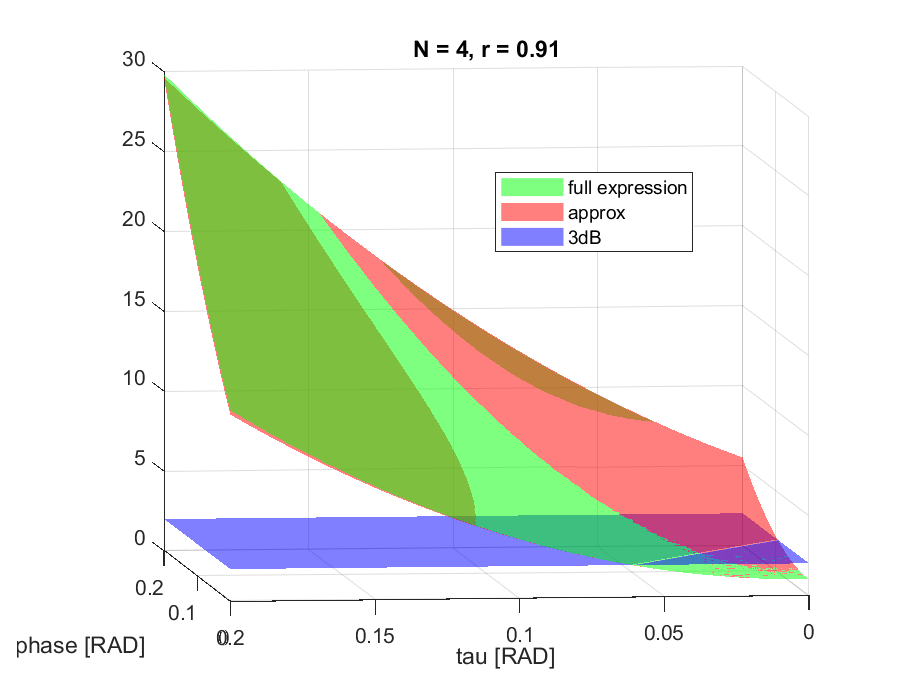
\includegraphics[width=0.9\linewidth]{./Media/spatial_IIR_MATLAB/beamwidth/BW_approx_validation.eps}
    \caption{Graphically comparing (\ref{eqn_arrayPerformance_beamwidth_fullEpxr}) and (\ref{eqn_arrayPerformance_beamwidth_approx}) for $N=4$ and $\rho=0.91$. The approximation seems to closely match the original expression.}
\end{figure}
Unlike the passive ULA case, it is evident from figure (\ref{fig_singleFreqFeedback_2ndTaylorNumericalValidation}) that the $4^{th}$ order terms are not needed for the evaluation of $\theta_{HPBW}$. In perfect phase alignment (i.e. $\Delta_{\tau}=0$), the u-space expression for the HPBW is $$u_{HPBW} =
\frac{
\left|1-\rho\right|
}{
\pi{d}
}
\lambda
\sqrt{\frac{
12
}{
\left(N-1\right)\left(\left(1+2r\right)N-4r+1\right)
}}.
$$
Comparing to the classic ULA beamwidth \cite{VanTrees2002DetectionIV}, thoroughly discussed in appendix \ref{appendix_theULABeamwidth}, we can express the improvement factor as
$$
\frac{
0.89\frac{\lambda}{ND}
}{
\theta_{HPBW,IIR}
}
=
\frac{0.89}{\left|1-\rho\right|}\sqrt{\frac{1+2r}{12}}
$$
\todo{TODO}
\textbf{Add graph of the improvement factor}
% \subsection{The pole-based design approach}
% In this approach, we look for setting the response "poles" which minimize the denominator, thus maximizing the overall response magnitude. To evaluate the beamwidth, we chose to allocate all of the system's poles in a single position such that 
% $
% 1-\vecnot{\beta}^{T}\vecnot{d}_{\theta}e^{-j\tau}
% =
% \left(e^{j\theta}-re^{j\theta_{s}}\right)^{N}
% $
% where $N$ is the number of array sensors and $r \in \left[0,1\right)$ enables us to avoid treatment of $\infty$-valued expressions. Next, we look for $\theta$ such that
% $
% \left|\frac{
% \frac
% {
% \vecnot{\alpha}^{T}\vecnot{d}_{\theta_{s}}
% }{
% \vecnot{\beta}^{T}\vecnot{d}_{\theta_{s}}
% }
% }{
% \frac
% {
% \vecnot{\alpha}^{T}\vecnot{d}_{\theta}
% }{
% \vecnot{\beta}^{T}\vecnot{d}_{\theta}
% }
% }\right|
% = \frac{1}{\sqrt{2}}
% $. Assuming that, like in classical IIR filter design theory, the numerator behaviour is significantly "slower" than the denominator's which results in $\vecnot{\alpha}^{T}\vecnot{d}_{\theta} 
% \approx
% \vecnot{\alpha}^{T}\vecnot{d}_{\theta_{s}}$ reults in
% \begin{align*}
%     \left|\frac{
%     \vecnot{\beta}^{T}\vecnot{d}_{\theta}
%     }{
%     \vecnot{\beta}^{T}\vecnot{d}_{\theta_{s}}
%     }\right|
%     &= \frac{1}{\sqrt{2}}
%     \\
%     \left|
%     \frac{
%     \left(e^{j\theta}-re^{j\theta}\right)^{N}
%     }{
%     \left(e^{j\theta}-re^{j\theta_{s}}\right)^{N}
%     }
%     \right|
%     &=
%     \left|
%     \frac{
%     \left(1-re^{j\left(\theta_{s}-\theta\right)}\right)
%     }{
%     \left(1-r\right)
%     }
%     \right|^{N}
%     \\
%     &=
%     \left|
%     \frac{
%     1+r^{2}-2r\cos{\left(\theta_{s}-\theta\right)}
%     }{
%     \left(1-r\right)^{2}
%     }
%     \right|^{\frac{N}{2}}
%     =
%     \left(\frac{1}{2}\right)^{\frac{1}{2}}
%     \\
%     \Rightarrow 
%     1+r^{2}-2r\cos{\left(\theta_{s}-\theta\right)}
%     &=
%     \left(1-r\right)^{2}2^{\frac{1}{N}}
%     \\
%     \cos{\left(\theta_{s}-\theta\right)}
%     &=
%     \frac{
%     1+r^{2}-\left(1-r\right)^{2}2^{\frac{1}{N}}
%     }{
%     2r
%     }
%     \\
%     \Rightarrow
%     \frac{\omega{D\left(cos(\theta_{g,s})-cos(\theta_{g,B})\right)}}{c}
%     &=
%     cos^{-1}
%     \left(
%     \frac{1+r^{2}-\left(1-r\right)^{2}2^{\frac{1}{N}}}{2r}
%     \right)
% \end{align*}.
% Therefore,
% \begin{equation}
%     \theta_{g,B} 
%     &= 
%     cos^{-1}
%     \left(
%     cos(\theta_{g,s})
%     -
%     \frac{c}{\omega{D}}
%     cos^{-1}
%     \left(
%     \frac{1+r^{2}-\left(1-r\right)^{2}2^{\frac{1}{N}}}{2r}
%     \right)
%     \right)
% \end{equation}
% Few observations can be derived from the $ \theta_{g,B} $:
% \begin{itemize}
%     \item $r\rightarrow{1}$ (i.e. setting the pole on the unit circle) causes $\theta_{g,B}\rightarrow\theta_{g,s}$ due to the $\infty$ valued response at $\theta_{g,s}$
%     \item The interval 
%     $
%     \left\{
%     \theta_{g,s}
%     \ \Bigg{|}\ 
%     cos(\theta_{g,s})
%     -
%     \frac{c}{\omega{D}}
%     cos^{-1}
%     \left(
%     \frac{1+r^{2}-\left(1-r\right)^{2}2^{\frac{1}{N}}}{2r}
%     \right)
%     <-1
%     \right\}
%     $, has no solution. In simulations, when evaluating such $\theta_{g,s}$ values, one can observe that the actual beampattern does not resemble the designed one due to the ULA geometric properties.
%     \item The number of sensors $N$ seems to have low impact on the beamwidth.
% \end{itemize}
\subsection*{Location of sidelobes and the rate of decrease}
Unlike the passive ULA case, it is clear from (\ref{eqn_arrPerformance_beamwidth_3dB}) that the positions of the feedback based beampattern sidelobes are affected both by the numerator and the denominator of $\Hr_{\dTheta}$. Considering the \coefSetName{} approach (i.e. single DOA enhancement), the denominator has only one single minima on the main lobe. Therefore, the sidelobes positions, same as the ULA case, are known \cite{VanTrees2002DetectionIV} to be 
\begin{equation}
    \label{eqn_CB_sidelobesLocations}
    \dTheta_{\coefSetName{},\text{sidelobes}} = \frac{\rBrace{2m+1}\pi}{N}\ \forall m\in\cBrace{1,2,\hdots}.
\end{equation}
Our initial interest is the first sidelobe (i.e. $m=1$), therefore we express the normalized beampattern at $\dTheta = \frac{3\pi}{N}$ (and setting $\dPhi=0$ for objective comparison). It can easily be verified that 
\begin{equation*}
    \Hr_{\frac{3\pi}{N}}
    =
    \frac{
    2\rBrace{1-r}^{2}
    }{
    \rBrace{N^{2}-2Nr}\rBrace{1-\cos{\rBrace{\frac{3\pi}{N}}}}+2r^{2}
    },
\end{equation*}
which for large $N$ values (as seen in Fig.~\ref{fig_firstSidelobeGain_CB}), can be well approximated by
\begin{equation*}
    \sqrt{\Hr_{\frac{3\pi}{N}}}
    \overset{N\gg1}{\approx}
    \frac{
    2\rBrace{1-r}
    }{
    3\pi
    }.
\end{equation*}
\begin{figure}[t!]
    \begin{center}
        \begin{overpic}[width=.75\linewidth, 
        %grid, 
        tics=10,trim=0 0 0 0]{./Media/spatial_IIR_MATLAB/arrayParameters/firstSidelobeGain_vs_N_various_r.eps}
            \put (6, 72){\footnotesize{$\Hr_{\frac{3\pi}{N}}{}$ - First sidelobe gain}}
            \put (20, 54) {\footnotesize{$r=0$ (i.e. no feedback)}}
            \put (20, 42) {\footnotesize{$r=0.3$}}
            \put (20, 33) {\footnotesize{$r=0.5$}}
            \put (20, 24) {\footnotesize{$r=0.7$}}
            \put (20, 14) {\footnotesize{$r=0.9$}}
            \put (-3, 50.5) {{$\frac{2\rBrace{1-0}}{3\pi}$}}
            \put (-3, 37.5) {{$\frac{2\rBrace{1-0.3}}{3\pi}$}}
            \put (-3, 28.5) {{$\frac{2\rBrace{1-0.5}}{3\pi}$}}
            \put (-3, 20) {{$\frac{2\rBrace{1-0.7}}{3\pi}$}}
            \put (-3, 12) {{$\frac{2\rBrace{1-0.9}}{3\pi}$}}
            \put (50, 2) {\footnotesize{$N$}}
        \end{overpic}
    \end{center}
    \caption{Plot of $\Hr_{\frac{3\pi}{N}}{}$ (i.e. the first sidelobe gain) vs. N for various $r$ values. The expected limit values (for large $N$) are presented as horizontal lines for each instance of $r$. Evidently, as expected, the gains tend to unite with the matching limits. $r=0$ is of special importance, being the reference for evaluation of the integrated feedback related improvement.}
    \label{fig_firstSidelobeGain_CB}
\end{figure}
It follows that, comparing to the known \cite{VanTrees2002DetectionIV} result of the passive ULA case (i.e. first sidelobe gain of $\frac{2}{3\pi}$), the first sidelobe gain improvement factor under the \coefSetName{} approach is
\begin{equation}
    \mu_{\text{first-sidelobe-gain,\coefSetName{}}} = \frac{1}{1-r}.
\end{equation}
Since the denominator magnitude, under the \coefSetName{} approach, is practically flat when not around the main lobe, the rate of sidelobes decay stays approximately the same as the numerators, which is similar to the known \cite{VanTrees2002DetectionIV} passive ULA sidelobe decay rate of $1/\rBrace{2m+1}$ (where $m$ is the sidelobe index).
\subsection*{Array directivity}
Another common measure for the array performance is the directivity \cite{VanTrees2002DetectionIV}, $\text{D}$. In the context of this work, considering the steer error scenario, it is defined as
\begin{equation*}
    \text{D}_{\coefSetName{}} = \frac{\Hr_{0}}{\frac{1}{2\pi}\int^{0}_{2\pi}\Hr_{\dTheta}\ d\dTheta},
\end{equation*}
measuring the ratio between the maximal array gain to the averaged gains in all directions. For uniformly weighted passive ULAs, assuming normalized beampattern, it is known \cite{VanTrees2002DetectionIV} that $D = N$.
\par Numerically sweeping various $\vBrace{N,r}$ sets, unveils that
\begin{equation}
    \text{D}_{\coefSetName{}} = \frac{r^{2}-\rBrace{N-1}r+N}{\rBrace{r-1}^{2}},
\end{equation}
matching the passive ULA result (i.e. $\evalat{D_{ULA}}{r=0}=N$), which leads to expressing the \coefSetName{} directivity improvement factor 
\begin{equation}
    \mu_{\text{D},\coefSetName{}}= \frac{r^{2}-\rBrace{N-1}r+N}{N\rBrace{r-1}^{2}}\overset{N\to\infty}{\to}\frac{1}{\rBrace{r-1}}.
\end{equation}
It is worth mentioning that for $\vBrace{r\to1,N\gg1}$ value sets, classic numerical approximations for the integral fail around $\dTheta\to0$ due to the the fact that both the numerator and the denominator tend to 0 (known to have a finite limit of 1 for $\dTheta=0$), forcing symbolic evaluation which was achieved using MATHEMATICA.